\section{Results}

\subsection{Main Finding: Extraction Rate Below Target}

The existence test (H-E1) \textbf{did not meet} the primary criterion. Overall extraction rate was 49.5\%, well below the 95\% target.

\begin{table}[h]
\centering
\begin{tabular}{@{}ll@{}}
\toprule
Component & Extraction Rate \\
\midrule
AS\_loc & 49.5\% \\
AS\_state & 2.7\% \\
AS\_causal & 15.5\% \\
\bottomrule
\end{tabular}
\end{table}

\begin{figure}[h]
\centering
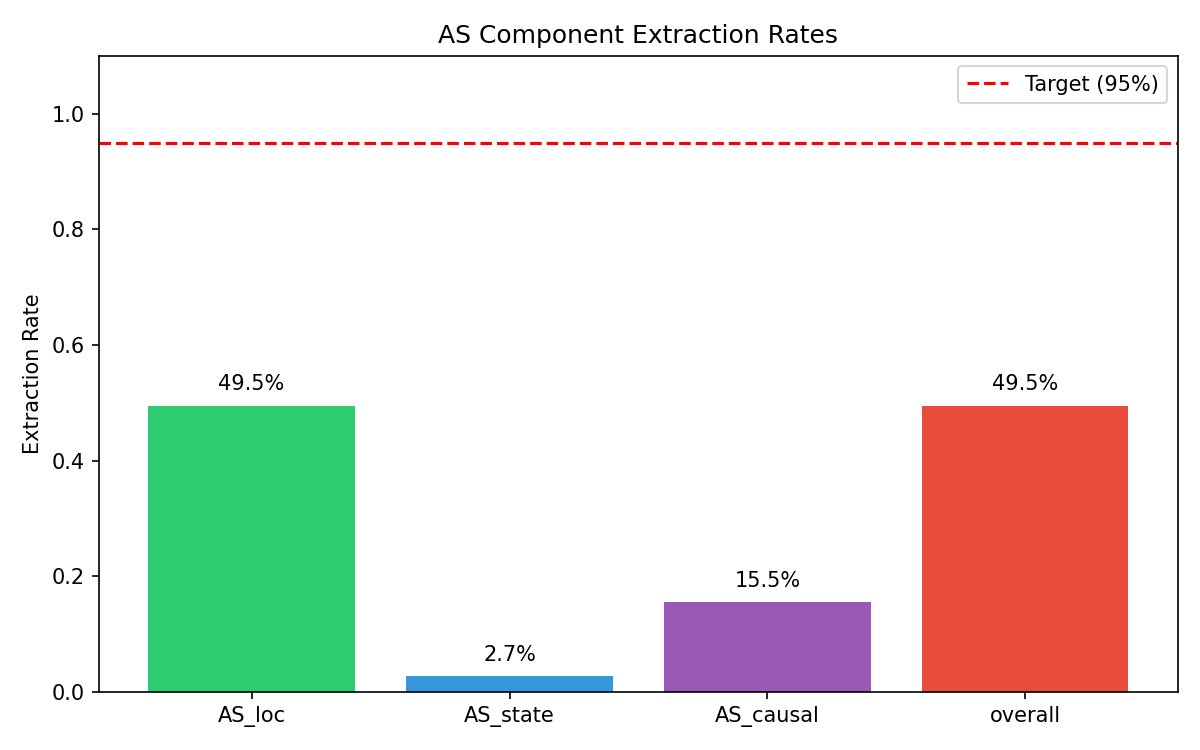
\includegraphics[width=\columnwidth]{figures/extraction_rate_bar.png}
\caption{AS component extraction rates showing 49.5\% overall extraction with near-zero state information (2.7\%).}
\label{fig:extraction_rates}
\end{figure}

\subsection{Error Type Distribution}

\begin{table}[h]
\centering
\begin{tabular}{@{}lrr@{}}
\toprule
Error Type & Count & Percentage \\
\midrule
Assertion & 341 & 53.4\% \\
Other & 171 & 26.8\% \\
Type & 116 & 18.2\% \\
Syntax & 5 & 0.8\% \\
\bottomrule
\end{tabular}
\end{table}

\textbf{Assertion errors dominate} (53.4\%) and produce minimal output without traceback frames, explaining the low extraction rate.

\subsection{AS Ordering Preserved on Extractable Subset}

\begin{table}[h]
\centering
\begin{tabular}{@{}ll@{}}
\toprule
Condition & Mean AS\_state \\
\midrule
C1 & 0.09 \\
C2 & 0.09 \\
C3 & 0.00 \\
C4 & 0.00 \\
\bottomrule
\end{tabular}
\end{table}

\textbf{Ordering C1$\geq$C2$\geq$C3$\geq$C4: PASS} (on the 49.5\% extractable subset)

\subsection{Component Independence}

All correlations $<$ 0.5, confirming components are reasonably independent.

\begin{figure}[h]
\centering
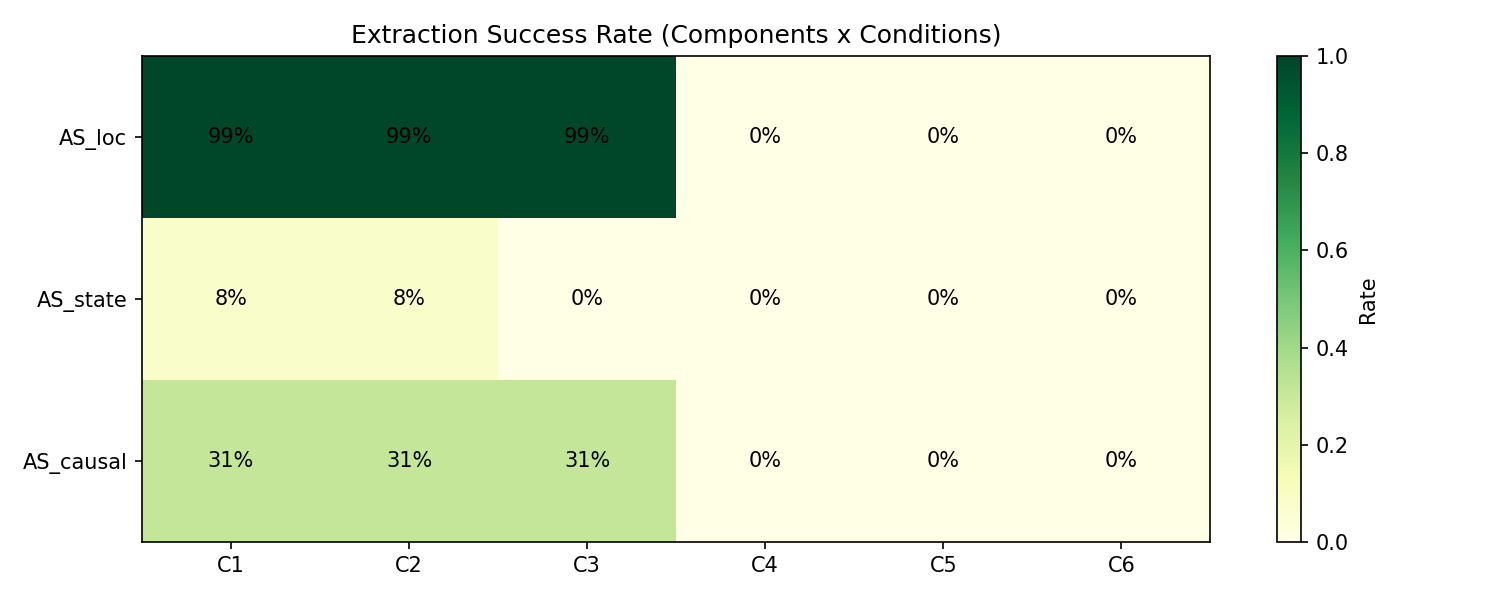
\includegraphics[width=\columnwidth]{figures/extraction_heatmap.png}
\caption{Components $\times$ conditions success matrix.}
\label{fig:heatmap}
\end{figure}

\begin{figure}[h]
\centering
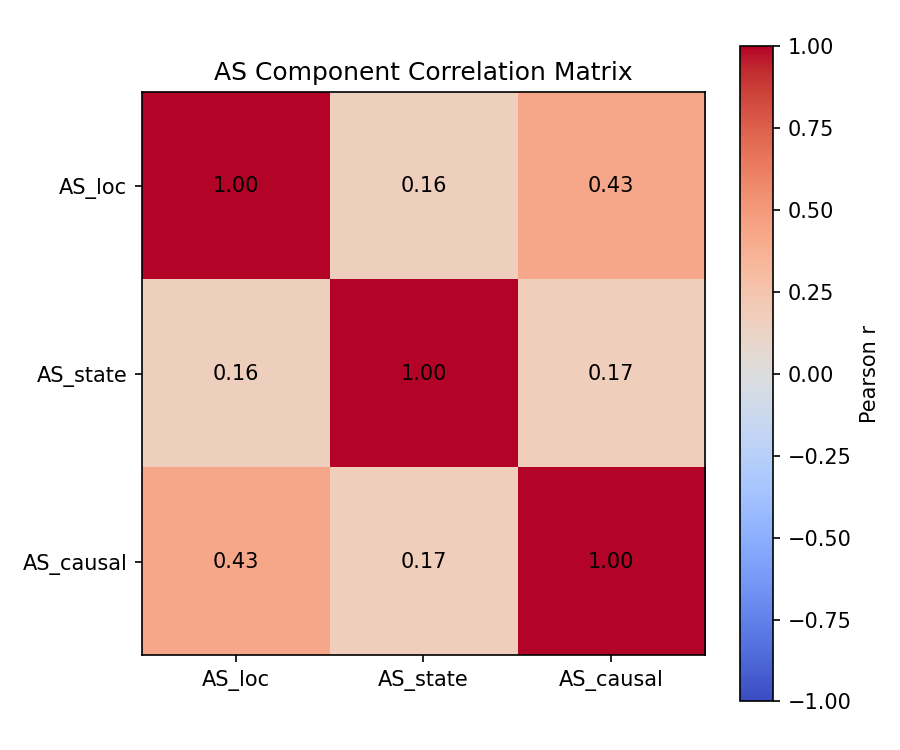
\includegraphics[width=\columnwidth]{figures/correlation_matrix.png}
\caption{Component correlation matrix demonstrating independence of AS dimensions.}
\label{fig:correlation}
\end{figure}
